% %%%%%%%%%%%%%%%%%%%%%%%%%%%%%%%%%%%%%%%%%%%%%%%%%%%%%%%%%%%%%%%%%%%%%%%%%%%%%%
%                           Making Mario Work Hard
% %%%%%%%%%%%%%%%%%%%%%%%%%%%%%%%%%%%%%%%%%%%%%%%%%%%%%%%%%%%%%%%%%%%%%%%%%%%%%%



% ------------------------------------------------------------------------------
% PACKAGES & DOCUMENT CONFIGURATION
% ------------------------------------------------------------------------------

\documentclass[11pt, a4paper, oneside]{report} % A4, 11pt font, one-sided
\usepackage[english]{babel}
\usepackage[utf8]{inputenc} %setlength{parskip}{0.7em}
\usepackage{bibentry} 
\usepackage[margin= 1.3in]{geometry}
\usepackage[colorinlistoftodos]{todonotes}
\usepackage{epigraph}
\usepackage{graphicx}
\usepackage{url}
\usepackage[nottoc]{tocbibind}

\linespread{1.1}

\begin{document}





% ------------------------------------------------------------------------------
% TITLE PAGE
% ------------------------------------------------------------------------------

\begin{titlepage}
    \begin{center}
        \vspace*{4cm}

        \Huge\textbf{Making Mario Work Hard}

        % \vspace{0.5cm}
        % Thesis Subtitle

        \vspace{2.5cm}

       \Large\textbf{Aaron Ceross}
       \\Supervisor: Dr. Benjamin Sach

        % \vfill
        \vspace{0.8cm}

        MSc Thesis Project\\
        COMSM3201 MSc Project, Computer Science
        \vspace{0.8cm}
        \vspace{0.8cm}

        % \includegraphics[width=0.4\textwidth]{university}

        % Department Name\\
        % University Name\\
        % Country\\
        \today

    \end{center}
\end{titlepage}


% ------------------------------------------------------------------------------
% Executive Summary
% ------------------------------------------------------------------------------

\chapter*{Executive Summary}

Blank at the moment

% ------------------------------------------------------------------------------
% ACKNOWLEDGEMENTS
% ------------------------------------------------------------------------------

\chapter*{Acknowledgements}

Blank at the moment

% ------------------------------------------------------------------------------
% TABLE OF CONTENTS
% ------------------------------------------------------------------------------

\tableofcontents





% ------------------------------------------------------------------------------
% CHP 1 --- INTRODUCTION
% ------------------------------------------------------------------------------

\chapter{Aims and Objectives}


\epigraph{``The obvious objective of video games is to entertain people by
surprising them with new experiences.''}{Shigeru Miyamoto}

\section{Background and motivation}

An NP-complete problem is one with a solution that can be \textit{verified}
quickly in polynomial time, though an existing solution is not readily known or
\textit{identifiable} \cite{cook1984can}. It has been proven that certain
classic video games, such as \textit{Super Mario Bros} \cite{Aloupis2012}, are
computationally hard in that the character could be made to solve an arbitrary
instance of a Boolean satisfiability problem (SAT). SAT is a type of NP-complete
problem in which the variables of the formula may be consistently replaced by
the values TRUE or FALSE in a way that the formula evaluates to TRUE, or
`satisfiable'.

The primary motivation of this research is to investigate the feasibility of the
video game medium as a teaching tool to visualise and demonstrate concepts in
computational complexity. This could be achieved through the evaluation of
different instances of SAT in a video game setting.\@ 

Computer science and mathematics can be quite daunting subjects for new students
and quite often the concepts may not be clear. The utilisation of video games as 
a medium to introduce the topic and concepts could be 

There are several challanges that need to be addressed in order for this method
to be feasible.


\section{Research aims and objectives}

% This project concerns the complexity of Mario which is known to be NP-
% Complete. To prove this it was shown that Mario could be forced to solve an
% (arbitrary) instance of the satisfying assignment problem (``SAT'') --- this
% is called a reduction. One computational problem is reducible to another
% problem if it is possible to efficiently solve the first one when provided
% with an efficient algorithm for solving the other. A problem in NP is
% determined to be NP complete if any problem in NP is reducible to it.The aim
% of this project is to implement a simple platform game and a level generator.
% The level generator should take an input to the SAT problem and convert it
% into a Mario level. The project should also include an AI player which can
% play these levels by choosing a suitable path using an existing SAT solver.

The aim of this project is to produce a game engine that is capable of
visualising and demonstrating concepts in computational complexity through the
evaluation of different instances of SAT.\@ The game engine would be able to
take an instance of SAT and generate a human-playable level that is
computationally hard. This level would then be able to be solved by a SAT
solver. The solution to the level would then be visualised on screen. In order
to fulfil this aim, the research project will implement a game engine through
achieving the following objectives: \\ 

\begin{enumerate}

  \item Develop a platform game in which the mechanics are NP-hard;
  \item Develop a level generator which converts an instance of SAT into a playable level;
  \item Develop a visualisation of the SAT solving these levels by choosing a suitable path;
  \item Evaluate level-generation and display of the SAT solver's decisions for
        efficiency and success against an established criteria or one developed
        during the project.

\end{enumerate}


% \section{Scope of the research review}

% As shown in the preceding section, the research being undertaken brings together
% a diversity of broad topic areas, which is challenging. Given the research aims
% and objectives described above, the scope of the research review is to
% understand the current state of research and development in the following areas:

% \begin{enumerate}

%   \item The principles and concepts of computational complexity which class a task or activity as
%   `difficult' or `hard'. This includes an assessment of the characteristics which define the
%   differing classes of complexity;

%   \item  The tests of computational complexity that prescribe the different classifications through
%   Boolean satisfiability. This includes how these tests may be applied to video games, with
%   particular focus on 2D platform games;

%   \item The generation of video game content in order to produce the problem instances as levels in
%   an accurate and efficient manner.

%   \item Assessing the means for implementing these divergent areas of research in order to produce a
%   bespoke game engine that realises the research aim.


% \end{enumerate}

As shown from the range of topics above, the areas being investigated are
expansive and multi-faceted. Therefore, this research review surveys those
elements most relevant for the implementation and development of the game engine
software.

\section{Thesis Structure}

This research project is divided between 66\% Type I (software development) and
34\% Type II (investigatory, research). The structure of this document reflects
this division in that the theoretical concepts are broadly introduced and
discussed insofar as relevant to the research aim. The discussion strongly
focuses on the  implementaiton and development challenges in realising these
concepts in the project.

Chapter 2 covers the fundamental concepts in computational complexity,
identifying which characteristics render a task difficult. The chapter discusses
the well-known P vs NP question and explains the NP-hardness complexity class.
Other classes which are later explored within the project are also demonstrated
and analysed. 

The overview of computational complexity provides the basis for the discussion
in Chapter 3 on Boolean Satisfiability problems and SAT solving software. In
addition to explaining the major features of SAT solvers, the chapter also
identifies SAT solvers which had been considered during the project's
development.

Chapter 4 relates to how video games can be classified as `hard', through use of
Boolean satisfiability solvers. An overview of relevant research explores the
models and proofs that have been utilised in making such classification. The
frameworks highlighted in this chapter will form the basis of a model for the
implementation of the game engine. After which, Chapter 5 turns the focus of the
research review to the generation of game content, particularly centred on game
levels.  This chapter critically examines methodologies and techniques.

In Chapter 6, the research review will consider the initial design
specifications and features of the implementation of the game engine. Discussion
will focus on utilising the outputs from this review in a viable game engine
model. Finally, Chapter 7 will draw conclusions from this initial research
review and discuss future areas of investigation.

%---------------------------------------------------------------------------------------------------
% CHP 2 --- COMPUTATIONAL COMPLEXITY AND VIDEO GAMES
%---------------------------------------------------------------------------------------------------

\chapter{Computational complexity theory}

\epigraph{``In general, it is much harder to \textit{find} a solution to a problem than to
\textit{recognize} one when it is presented''}{Stephen A Cook \cite{cook1984can}}

\section{Fundamental concepts}

\subsection{Definitions}

The goals of the research project are to visualise computational complexity
through video games. Therefore, the literature review begins with identifying
the relevant key concepts in computational complexity theory in order to
understand what characteristics makes a problem computationally hard.

Computational complexity theory is concerned with assessing and classifying the
difficulty of defined tasks as well as the relationship between such tasks.
Within computational complexity, there exist different types of problems, termed
\textit{complexity classes}. Complexity classes rank the difficulty of differing
types of problems. Of the many types of problems which can exist in
computational complexity theory, the two fundamental types this research project
is interested in are (\textit{i}) decision problems and (\textit{ii}) search
problems. The importance of the distinction between these two types will be made
clearer when discussing Boolean satisfiability (Chapter 2) and procedural
content generation (Chapter 5).

\subsubsection{Decision problems and search problems}

A decision problem is a binary choice one wherein, on an infinite set of inputs,
the question may be answered `\textit{yes}' or `\textit{no}'  It is common  to
define the decision problem equivalency as: ``the set of inputs for which the
problem returns \textit{yes}''. Most problems may be reduced to a decision
problem \cite{kendall2008survey}, which is important in that the determination
of whether a solution exists or not is required in order to solve the
complementary search problem \cite{Goldreich:2008}.

Search problems represent a significant area of research in computer science
(citation needed), covering topics such as sorting and identifying the shortest
path \cite{Goldreich:2008}. A search problem consists of the identification of a
solution from a set of solutions (possibly infinite or empty). Therefore, given
an instance of a search problem, a solution must be found or return a
determination that no solution exists in such instance.

\subsection{Survey of complexity classes}

\subsubsection{P and NP}

The two fundamental complexity classes relevant for this research project are
\textbf{P} and \textbf{NP}\@. The P (polynomial) class of problems contain those
decision problems that are often described as `easy' problems
\cite{kendall2008survey} as the time required to solve such problem has an
upper- bound that scales by a polynomial function of the input
\cite{sipser2012introduction}. The other complexity class, NP (non-deterministic
polynomial), relates to those problems that do not have an efficient way of
finding a solution but can have a solution verified in polynomial time
\cite{Goldreich:2008, Papadimitriou:2003:CC:1074100.1074233}.

% Therefore:
% \\

% \centerline{T(\textit{n}) = O(\textit{n}$^k$)}

% Where \textit{T}


\subsubsection{P vs NP Problem}

The P vs NP problem refers to search problems to which there exists an efficient
algorithm that given a solution to a given instance determines whether or not
the solution is correct\cite{sipser2012introduction,Goldreich:2008,kendall2008su
rvey,du2011theory}.\footnote{This is also sometimes described as the P vs NP
Question in literature} Although any given solution to an NP-complete problem
can be verified quickly (in polynomial time), there is no known efficient way to
locate a solution in the first place. A distinguishing characteristic of of NP-
complete problems is that there is no known efficient solution to them
\cite{Goldreich:2008}. That is, the time required to solve the problem using any
currently known algorithm increases very quickly as the size of the problem
grows.

\begin{figure}[h!]

  \centering
    
\includegraphics[scale=0.45]{pnp}
  \caption{Euler diagram illustrating the relationship between P and NP \cite{esfahbod:euler}.}
  \label{Euler}
\end{figure}


Proving that P = NP or P $\neq$ NP is one of the most important open questions
in theoretical computer science and has been described as one of seven principal
unsolved problems in the field of mathematics \cite{devlin2002millennium}. The
implications of P = NP are far-reaching. If it were possible to demonstrate that
P = NP (i.e. all NP problems can be solved in polynomial time), then it would
then be possible to solve difficult problems in polynomial time (see
Figure~\ref{Euler}). For every problem that has an efficiently verifiable
solution, that same solution could also be efficiently identified. While the
problem is still being researched and open to debate, there is wide belief that
P $\neq$ NP is more likely than P = NP \cite{Gasarch:2012:GCS:2261417.2261434}.


% Search problems, for example, are not known to be solveable in polynomial time.


\subsubsection{NP-hard}

A problem is considered to be classed as \textbf{NP-hard} if the solution's
algorithm may be adapted to solve any problem in NP. By extension, this will
then include all problems in P, which are contained within NP. It should be
noted that not all NP-hard problems fall within NP nor are NP-hard problems
necessarily decidable problems
\cite{sipser2012introduction,Goldreich:2008,kendall2008survey,du2011theory}.

\subsubsection{NP-complete}

When a problem is classed as both NP and NP-hard is said to be \textbf{NP-
complete} and are considered to be the hardest problems in NP
\cite{sipser2012introduction,Goldreich:2008,kendall2008survey,du2011theory}. A
problem that is NP- complete can have every other problem in NP reducible to it
\cite{papadimitriou2003computational}. `Reduction' in this sense that there
exists an algorithm in P that change a problem into another instance
\cite{du2011theory}.

\subsubsection{PSPACE}

Another relevant complexity class to this research review is \textbf{PSPACE}, as
some games have been proven to be in this class \cite{DBLP:conf/fun/Forisek10,
demaine2002push}.\footnote{Please refer to Chapter 3 of this research review for
further information.} PSPACE refers to decision problem which may be solved with
an amount of space polynomial in the size to its input
\cite{sipser2012introduction}.

\section{Chapter summary}

This chapter has identified the relevant complexity classes and problems in
order to establish that video games are computationally complex in Chapter 4. In
the next chapter, these concepts will be used to show how problem instances may
be proven to be NP-complete through the use of Boolean expressions. This will
provide the foundation for being able to develop a game engine which produces
computational hard levels in a video game.


%---------------------------------------------------------------------------------------------------
% CHP 3 --- BOOLEAN SAT SOLVERS
%---------------------------------------------------------------------------------------------------

\chapter{Boolean satisfiability problems}

\epigraph{``It is not of the essence of mathematics to be conversant with the
ideas of number and quantity.''}{George Boole}


This chapter provides insight into the hardness of Boolean satisfiability
problems (or SATs). SATs are the basis for proving the hardness of video games
so understanding how they work is important. During the implementation, SAT
solvers (programs that solve instances of SAT) will be used to run tests through
the constructed game.

\section{Principle concepts and definitions}

A Boolean formula is a logic expression with variables that have a value of
either TRUE or FALSE. These formulae also contain logical connectives, which
subscribe to an order of precedence: negation ($\neg$), conjunction($\wedge$),
disjunction ($\vee$), implication ($\leftarrow$), and equivalence
($\leftrightarrow$) \cite{balyo2010solving,gomes2008satisfiability}.

Formulae are constructed through literals, which is a variable (e.g. \textit{x}
or \textit{y})  or its negation (e.g. \textit{x} or $\neg$\textit{x}) joined
together in clauses (e.g. \textit{x}). Of these constructions, the conjunctive
normal form (CNF) is of particular importance, especially in relation to finding
solutions to satisfiability problems, particularly those solving methods based
on DPLL algorithm \cite{gomes2008satisfiability} (See Section X below for
further discussion). To be in CNF, a formula must a conjunction of clauses,
wherein those clauses are a disjunctive of literals. For example:

\centerline{(x $\vee$ $\neg$y) $\wedge$ ($\neg$x $\vee$ z $\vee$ y) $\wedge$ ($\neg$z $\vee$ x)}

\par  \noindent The example above is a conjunctive normal form with three clauses (joined together by $\wedge$ (AND)) containing three literals (x, y, z).

\section{Boolean Satisfiability problem and NP-completeness}

The Boolean satisfiability problem (SAT) is the problem of determining if there
exists an assignment that satisfies a given Boolean formula. In order for such
assignment to be \textit{satisfiable}, the variables' values are replaced
constantly with TRUE or FALSE until the formula evaluates to TRUE. Where no such
assignment is possible (i.e. the formula evaluates to FALSE in all
combinations), the formula is determined to be \textit{unsatisfiable}
\cite{balyo2010solving,gomes2008satisfiability}. Therefore, given a CNF formula
\textit{F}, SAT may be posed as: does \textit{F} have a satisfying assignment?

This question has an important place in computer science as it was the first
problem proven to be NP-complete \cite{cook1971complexity}.\footnote{While this
is often described as \textit{Cook's Theorem} it had been independently verified
in \cite{levin1973universal} and is more accurately termed the \textit{Cook-
Levin Theorem}} In solving a SAT problem, the question involves not only
providing a yes or no, but also in finding an actual solution to the assignment
\cite{zhang2002quest}. Specialised software, SAT solvers (discussed in Section
3.2.2 below), provide these solutions, if one exists.

\subsection{Examples of SAT reductions}

Three-satisfiability or 3SAT is the SAT reduction is most relevant for the
research project as it has been used to demonstrate the NP- completeness of 2D
platform games  \cite{Aloupis2012}. In 3SAT, there may only ever be three
literals in each clause and at least of of the literals contain a value of TRUE
in order to achieve satisfiability \cite{balyo2010solving}.There is a variant of
the 3SAT, exactly 1-3-satisfiability or 1-in-3SAT above reduction wherein the
each clause must contain \textit{exactly} one literal \cite{balyo2010solving,
du2011theory}.


\section{SAT solvers}

SAT solvers are software that given a SAT instance can either find a solution,
which would be a satisfying variable assignment or prove that no solution exists
\cite{zhang2002quest}. There are also stochastic methods based on local search
may be able to find satisfiable instances in a fast manner but are unable to
prove that an instance is in fact unsatisfiable \cite{gomes2008satisfiability}.


\subsection{The DPLL algorithm}

The Davis-Putnam-Logemann-Loveland (DPLL) algorithm \cite{davis1962machine} is a
complete, systematic search algorithm which is based on backtracking. The DPLL
algorithm (see Figure~\ref{DPLL}) is able to decide the satisfiability of a CNF
SAT reduction as well as identify the satisfying assignment. It can also show
that a given Boolean formula is unsatisfiable. The algorithm achieves these
results through the use of branching and where clauses are found to be FALSE,
removes these from its search space.

\begin{figure}[h!]

  \centering
    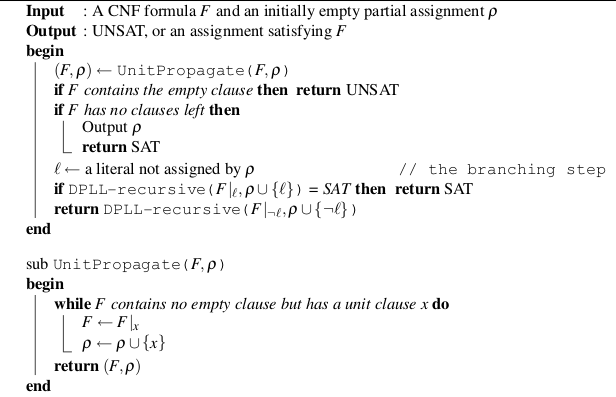
\includegraphics[scale=0.47]{dpll}
  \caption{DPLL in pseudo-code. Adapted from \cite{balyo2010solving,gomes2008satisfiability}.}
  \label{DPLL}
\end{figure}

The DPLL algorithm works with the CNF of a propositional logic expression (as
described in Section 3.1 above). Given that any formula may be converted into
CNF through the addition of new variables corresponding to the sub-formulae
\cite{tseitin1983complexity,Goldreich:2008}, DPLL may used to in all cases.

\section{Available SAT solvers}

The following SAT solvers have been identified as being potentially viable for
the research project: MiniSAT\footnote{http://minisat.se}
\cite{sorensson2005minisat};
zChaff\footnote{http://www.princeton.edu/~chaff/zchaff.html}
\cite{marques1999impact}; jerusat \cite{nadel2002jerusat}; BerkMIN
\cite{Goldberg20071549};
Glucose\footnote{http://www.labri.fr/perso/lsimon/glucose/}
\cite{audemard2009glucose}. These may be scope for the research to
simultaneously compare the efficacy of different solvers in varying conditions
in the research project (e.g. size of level).ow


\subsubsection{Features of modern DPLL-based SAT solvers}

Modern DPPL-based SAT solvers are readily available and useful for this project.
There are currently a number of highly scalable SAT solvers, all based on the
classic DPLL search framework. These solvers, now also known as conflict-driven
clause learning (CDCL) solvers, can generally handle problem instances with
several million variables and clauses \cite{katebi2011empirical}. In the section
below, a collection of important features have been identified and have
relevance for the research project.

\begin{enumerate}


  \item \textbf{Selection heuristic} : \indent Also termed the `decision
strategy', this is the procedure of \textit{how} variables are selected and
assigned values. This aspect varies the most between different solvers can
significantly impact the efficiency of a solver
\cite{marques1999impact,gomes2008satisfiability, zhang2002quest}. There are a
range of strategies that can be employed including: Maximum occurrence in
clauses of minimum size heuristic \cite{jeroslow1990solving}, Bohm's heuristic
\cite{marques1999impact}, dynamic largest individual sum heuristic
\cite{marques1999grasp}, variable state independent decaying sum
\cite{moskewicz2001chaff}.

  % \subitem \textbf{Maximum occurance in clauses of minimum size heauristic} \cite{jeroslow1990solving}
  % \subitem \textbf{Bohm's heuristic} \cite{marques1999impact}
  % \subitem \textbf{Dynamic largest individual sum heauristic} \cite{marques1999grasp}
  % \subitem \textbf{Variable state independent decaying sum} \cite{moskewicz2001chaff}

%%%%%%%%%%%
%  is one of the features that vary the most from one
% SAT solver to another. Also referred to as the decision strategy, it can have a significant impact
% on the efficiency of the solver (see e.g. [160] for a survey).

% is one of the features that vary the most
% from one SAT solver to another. Also referred to as the decision strategy, it can have
% a significant impact on the efficiency of the solver (see e.g. [160] for a survey). The
% commonly employed strategies vary from randomly fixing literals to maximizing a
% moderately complex function of the current variable- and clause-state, such as the


%  MOMS (Maximum Occurrence in clauses
% of Minimum Size) heuristic [121] or the BOHM heuristic [cf. 32].

%One could select and fix the literal occurring most frequently in the yet unsatisfied clauses (the DLIS (Dynamic Largest
% Individual Sum) heuristic [161]), or choose a literal based on its weight which periodically decays
% but is boosted if a clause in which it appears is used in deriving a conflict, like in the VSIDS
% (Variable State Independent Decaying Sum) heuristic [170].

% Newer solvers like BerkMin \cite{Goldberg20071549}, , and RSat [184] employ
% further variations on this theme.

  \item \textbf{Clause learning} :  This method allows the solver to learn the
causes of unsatisfiability (sometimes termed `conflict') in clauses, using this
information to minimise the search space \cite{biere2009conflict}. When a
conflicting clause is encountered, the solver will needs try  to identify the
cause of a conflict and attempt to resolve it. This is achieved by asserting
that a solution does not exist in the particular search space, backtrack
(undoing the previous decisions) and continuing the search in a new one.
\cite{zhang2002quest}. This feature has been identified as one that improves the
underlying DPLL algorithm \cite{zhang2002quest,gomes2008satisfiability}.

  \item \textbf{Conflict clause minimization} Een and Sorensson
\cite{sorensson2005minisat} had first explored the use of this method in their
\texttt{MiniSat} solver. By utilising subsumption resolution, the size of the
learned conflict is minimised through the removal of literals that are implied
to be FALSE when the rest of the literals in the clause are FALSE
\cite{zhang2002quest}. This increased efficiency come with an increased
computational cost \cite{gomes2008satisfiability}.

  \item \textbf{Conflict-directed backjumping} : \indent Stallman and Sussman
\cite{stallman1977forward}   proposed a method to allow a solver to backtrack
directly to a decision-point \textit{p} if the variables at level \textit{p} or
lower are causing conflict. The assumption is therefore that there is no
solution to be found in this search space. It is agreed that this provides
greater efficiency and completeness to the procedure
\cite{gomes2008satisfiability}.


  \item \textbf{Fast backjumping} : Gomes \textit{et al}.
\cite{gomes2008satisfiability} describe this feature as allowing for a solver to
directly go to a lower decision level if even one branch in the search space is
in conflict. The authors note that this may not always increase efficiency
however. The branch at depth level \textit{d} is not marked as unsatisfiable but
rather a new variable and value is selected for that level, continuing with a
new clause. There has been some experimental work that suggests an increase in
solving efficiency \cite{gomes2008satisfiability, kottler2010sat}.

  \item \textbf{Watched literals scheme}:  This feature monitors two classes of
literals in an unsatisfied clause: TRUE or unassigned \cite{moskewicz2001chaff}.
As an empty clause will cause the DPLL to stop, This feature had been introduced
in the the \texttt{zChaff} solver and is utilised by many other solvers due to
the efficiency of the constraint propagation \cite{gomes2008satisfiability}.
This somewhat of an advancement of the `lazy data structures' which had been
introduced by the \texttt{Sato} solver \cite{zhang1997sato}. This feature has
furthered development of clause learning
\cite{zhang2002quest,gomes2008satisfiability}.


  \item \textbf{Assignment stack shrinking} : In the \texttt{Jerusat} SAT solver
\cite{nadel2002jerusat}, Nadel had introduced this feature which is based on
conflict clauses. Assignment stack shrinking servers to make the search area
more local by `shrinking' the conflict clause once it reaches a set threshold
\cite{Nadel:2010:ASS:2164073.2164111}. The `shrinking' is achieved by finding
the lowest decision level that is less than the immediate higher level by at 2.
The solver will then backtrack to this level and where possible, sets unassigned
literals of the clause to FALSE \cite{Nadel:2010:ASS:2164073.2164111}.


  \item \textbf{Randomized restarts} : This provides that the clause learning
algorithm can restart   the branching process from decision level 0 while
retaining all the learned clauses \textit{et   al}. \cite{gomes1998boosting}.
Pioneered \texttt{zChaff} \cite{moskewicz2001chaff} many modern   SAT solvers
utilise highly aggressive restarts strategies, even below 20 backtracks, as it
demonstrably lowers the solution time \cite{gomes2008satisfiability}.

\end{enumerate}


\section{Chapter summary}

Boolean satisfiability is the foundation for proving NP-hardness and NP-
completeness for the project, as will be demonstrated in the next chapter. The
availability of SAT solvers is also useful in order to try and test different
ones with the research project's game engine. Currently in the available
literature, there is very little research in this regard to the subject of
linking SAT solvers and video game engines, therefore representing a fertile
ground for development with this research project. The issue may be that these
solvers will not scale well with the game engine. In that respect, Brummayer et
al. \cite{brummayer2010automated} developed `fuzz testing' techniques which
allow for debugging errors in larger SAT instances. These techniques are useful
in ensuring the scalability of the SAT solver when attempting to solve large
levels.




% ------------------------------------------------------------------------------
% CHP 3 --- Computational complexity and video games
% ------------------------------------------------------------------------------

\chapter{Computational complexity and the hardness of (video) games}

\epigraph{``I strongly approve the study of games of reason, not for their own
sake, but because they help to perfect the art of thinking.''}{Gottfried
Wilhelm Leibniz}

\section{Overview}

Having established the concepts and means of testing for certain classes of
computational complexity in the previous chapters, this chapter will address the
assessment of complexity in video games. There is a growth of interest and
research in analysing `mainstream' video games, including two- dimensional (2D)
platform games  \cite{viglietta2014gaming, DBLP:conf/fun/Forisek10, Aloupis2012,
Smith:2008:FAP:1401843.1401858}. This chapter will identify the characteristics
and tests required to class a game as computationally hard. This will inform the
design considerations of the research project in Chapter 6.

Puzzles and games have long been a subject of complexity research with many
games being found to be at least within NP-hard \cite{kendall2008survey}. This
is often based on the assumption that P $\neq$ NP \cite{demaine2001playing}. The
list includes a variety of grid and block placement games, wherein a player
manoeuvres a block around a map to a specified location, such as
\textit{Minesweeper}\cite{kaye2000minesweeper} and
\textit{Tetris}\cite{demaine2003tetris}. Titles such as \textit{Sokoban},
\textit{Push} and \textit{PushPush}, which have been shown to be not only NP-
hard \cite{demaine2000pushpush}, but also PSPACE-hard
\cite{culberson1999sokoban, dor1999sokoban}. In the case of \textit{PushPush},
there have been proofs of NP-hardness not only in 2D but in 3D as well
\cite{o1999pushpush}. More recently, Gual\`{a} \textit{et al}. have demonstrated
that a number of `match-three' games, grid-based games which are popular on
mobile devices, such as \textit{Candy Crush Saga} and \textit{Bejewled} are NP-
hard \cite{DBLP:journals/corr/GualaLN14}.

The current trend in this field is to assess classic franchises such as
\textit{Prince of Persia}, and \textit{Donkey Kong Country}. These studies are
more relevant to the research project as visualisation will utilise a 2D
platfomer resembling a game like \textit{Super Mario Bros}.


\section{2D platform games}

The research project focuses on developing a two-dimensional (2D) platform game
and thus the proof for NP-completeness is of particular interest. These games
are (very often) single-player games wherein the player traverses levels in
order to proceed to the next level. A `level' is a virtual spaces in which the
player character can manoeuvre and interact \cite{Burgun:2012}. The player's
game-play is influenced by the physics of the world, which often mean a
limitation of jump height and distance \cite{Burgun:2012}.

\subsubsection{Characteristics of 2D games}

In an examination of 2D platform games, a list of common puzzle elements found within the genre
\cite{Smith:2008:FAP:1401843.1401858,DBLP:conf/fun/Forisek10}. These include:

\begin{itemize}

  \item \textbf{long fall}: the maximum height from which the player character may fall without
                            receiving damage.

  \item \textbf{door opening}: the game world may include a variable number of doors and
                               suitable mechanisms to open them

  \item \textbf{door closing}: the game world contains a mechanism to close doors and a way for the
                               player to trigger the mechanisms

  \item \textbf{collecting items}: a set of items the player collects as part of the game. These may
                                   be necessary or optional content.

  \item \textbf{enemies}: Navigating the level may be made more challenging by having `enemy'
                          characters that must either be avoided or defeated by the player

\end{itemize}


\subsection{Characteristics of NP-hard games}

These above elements can be modeled into Boolean satisfiability problems, which
are known to NP- complete \cite{DBLP:conf/fun/Forisek10, cook1971complexity}.
The proofs of video games rely on this analogy and if a proof then removes
certain game elements, it is expected that the complexity of that game is
reduced \cite{viglietta2014gaming}.

Viglietta \cite{viglietta2014gaming} surveyed several classic video games games
published between 1980 and 1998, identifying general common elements and schemes
in video games that class them as computationally hard. These include
collectable items, activation of pathways (e.g.by key or button) by, or the
ability to destroy paths. Fori\v{s}ek \@\cite{DBLP:conf/fun/Forisek10} further
identifies several features specific to 2D platform video games which provide
for complexity, with particular focus on \textit{Prince of Persia}. In the work,
he posits a number of meta theorem, of which four are particularly relevant for
the research project:

\begin{itemize}

  \item \textbf{Meta-theorem 1}: A 2D platform game where the levels are constant and there is no
                                time limit is in P, even if the collecting items feature is present.

  \item \textbf{Meta-theorem 2}: A 2D platform game where the collecting items feature is present
                                 and a time limit is present as part of the instance is NP-hard.


  \item \textbf{Meta-theorem 3}: Any 2D platform game that exhibits the features long fall and
                                 opening doors is NP-hard.


  \item \textbf{Meta-theorem 4}: Any 2D platform game that exhibits the features long fall, opening
                                 doors and closing doors is PSPACE-hard.

\end{itemize}


Following the criteria above, it can be demonstrated that many platform games are not only able to be
classified as NP-hard but even PSPACE-hard in some cases.

Aloupis \textit{et al} \cite{Aloupis2012} surveyed the complexity of classic
Nintendo franchises by considering that the games are essentially a decision
problem of reachability: ``given a level, is it possible to reach the goal point
\textit{t} from the start point \textit{s}''? The authors also review subsequent
\textit{Super Mario Bros} titles as well as other platform games such as
\textit{Donkey Kong Country}.

In the work, the authors had generalised the map size and left all other
elements of the game in the original settings. The proofs in \cite{Aloupis2012}
rely on a reduction of the game to 3SAT and the `level' was modelled to the
problem instance. This represents two potential points of difference from the
current research project. First, the research goal is to develop a means to
generate large levels and scale accordingly. Secondly, further reductions aside
from 3SAT may be explored.  \\

\begin{figure}[h!]

  \centering
    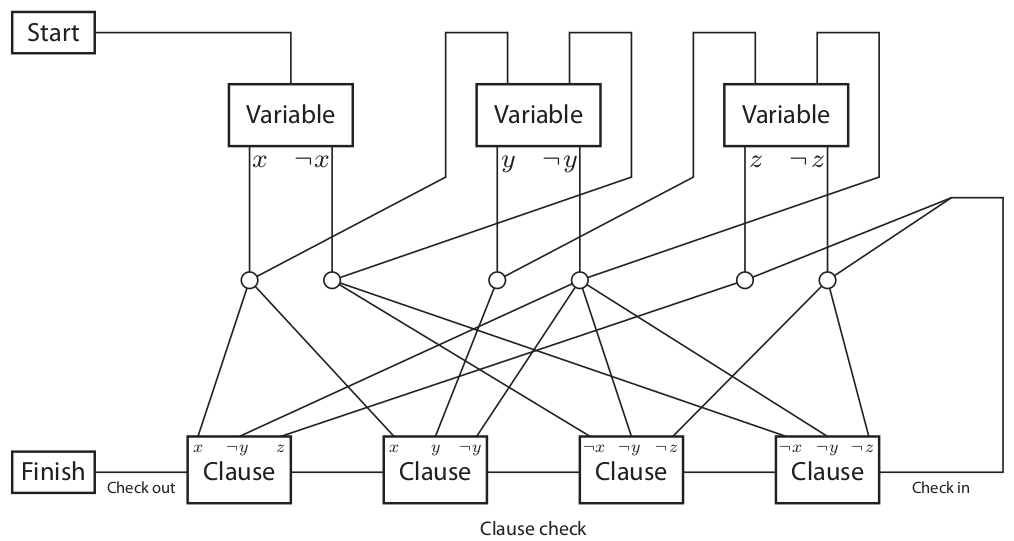
\includegraphics[scale=0.35]{aloupis_nphardness}
  \caption{Framework for NP-hardness \cite{Aloupis2012}.}
  \label{NP_hard}
\end{figure}

The framework for proving NP-hardness of games (see Figure~\ref{NP_hard}) is
reduced from 3SAT (described in Section 3.2.1 of this review). The player begins
the level at the \texttt{START} gadget and then traverses through variable
gadgets. A \textit{variable gadget} requires the player to make an choice, which
amounts to TRUE (\textit{x}) or FALSE (\( \neg \)\textit{x}) for the values in
the formula. These decisions allows the player to follow paths leading to
\textit{clause gadgets}. A clause gadget creates a permanent state change and as
a consequence, the player cannot access other paths connecting to that gadget.
As can be seen in the framework above, there are several areas of potential
crossover. To prevent such occurrence, \textit{crossover gadgets} prevent a
player from switching paths.

Once the player has passed through all the variable gadgets, the player can proceed to the
\texttt{FINISH} through a clause check path. This can only be successfully traversed only if every
clause gadget has been unlocked.


% \subsection{Proving a platformer is PSPACE-hard}

% % \subsubsection{\textit{Super Mario Bros}}

% % The construction of the games requires that that player character begins in a \texttt{Start} gadget
% % wherein the state requirement can be satisfied. In the case of \textit{Super Mario Bros}, the
% % \texttt{Start} gadget is a `Super Mushroom' that allows Mario to be in a large state, which is
% % necessary to reach the \texttt{Finish} gadget.

% \subsubsection{\textit{Donkey Kong Country}}

\section{Chapter summary}

The frameworks provided by \cite{Aloupis2012} give a comprehensive model for the
project's implementation. Modelling these gadgets to SAT clauses will form a
significant area of the research project's work. By utilising the metatheorms
provided by Fori\v{s}ek \cite{DBLP:conf/fun/Forisek10}, it may be possible to
incorporate other complexity levels including PSPACE-hard.

Having established how a 2D platformer may be classed as NP-hard (or even
PSPACE- hard), the focus of the literature review shifts to the details of how
these levels/problem instances will be generated, explored in the next chapter.


%%%%%%%%

% - for introduction to NP and concepts and classes – [10]

% - NP complete games feature levels whose solution demands some degree of ingenuity but such levels
% - are usually solved within a polynomial number of 'manipulations', and the challenge is to find
% - them. In contrast the additional complexity of a PSPACE-complete game seems to reside in the
% - presence of levels whose solution requires an exponential number of manipulations, and this may be
% - perceived as a nuisance by the player, as it makes for tediously long playing sessions.

% - several open problems remain for further research: whenever on the hardness of a game is proved
% with respect to some complexity class, the implied question is whether the game is also complete for
% that class. Indeed, the computational complexity of a game is expected to dramatically drop if some
% 'critical' elements are removed from its levels. It is interesting to study the 'complexity
% spectrum' of a game, as a function of the game parameters that we set. This has been done for the
% Lemmings game.

% - a problem instance will be a 'level' of the game

% -  the description of a level includes the position of every relevant game element, such as wall,
% -  items, character starting location. The question is always whether or not a given level can be
% -  'solved' under certain conditions, such as losing no lives. The exact definition of 'solvability'
% -  is highly game-dependent, and can range from reaching an exit location, to collecting some items,
% -  to defeating certain enemies.

% - all the metatheorems that follow yield hardness results under the assumption that certain game
% - elements are present in a given game.





% Meta theorem 3: Any 2D platform game that exhibits the features long fall and opening doors is NP-
% hard.  We will show how to reduce 3-CNF-SAT to such a game. The main idea of the proof is that the
% door opening mechanism can be used for a non-local transfer of information. Given an instance of 2
% -CNF-SAT, we can construct an instance of the game as follows: The instance will be divided into two
% parts: the key part, where the character starts, and the door part it reaches after exiting the key
% part. The door part will be a vertical concatenation of door gadgets (fig 1 left), each
% corresponding to a single clause in the 3-CNF-SAT instance. FORMULA pg. 3




%%%%%%%%%%%%%%%%%%%%%%%%%%%%%%%%%%%%%%%%%%%%%%%%%%%%%




%%%%%%%
% The player starts in the “start” gadget, which allows one to set up initial state requirements. For
% instance, in Super Mario Brothers, the start provides you with a mushroom, and you cannot get to the
% finish without being able to break blocks by jumping under them, which requires the mushroom power-
% up. Each “variable” gadget requires the player to make a variable assignment in such a way that the
% player can never return to that gadget to make a different decision. Then each “clause” gadget can
% be “unlocked” in some way, and each clause gadget can only be visited by the player once the player
% has chosen a satisfying variable assignment for that clause. Once the player has visited all
% variable gadgets, he goes to the “check in” area, and can travel back through all of the clauses to
% the finish if and only if he unlocked every clause. The crossover of the paths in the picture above
% requires another gadget to ensure that the player cannot switch paths (the details of this are in
% the paper).

% Note that if the player can only enter through one of the three columns at the top, then the only
% thing he can do is kick a red koopa shell down so that it breaks the blocks, unlocking the way for
% Mario to pass underneath at the end. Note that Mario cannot win if he falls from the top ledge
% (since must always remain large, he can’t fit through a one-tile-high entryway). Further details
% include the hole at the bottom, in which any stray koopa shell will necessarily fall, but which
% Mario can easily jump over. We recommend reading the entire paper, because it goes into all of the
% necessary details of the construction of the gadgets for all of the games.

%%%%%%%%%%%%%%%%%%%%%%%%%%%%%%%%%%%%%%%%%%%%%%%%%%%%%%






%%%%%

% General framework for proving the NP-hardness of platform games. The framework reduces from the
% classic NP-complete problem 3-SAT\@: decide whether a 3-CNF Boolean formula can be made TRUE by
% setting the variables appropriately. The player's character starts at the position labelled Start,
% then proceeds to the Variable gadgets. Each Variable gadget forces the player to make an exclusive
% choice of TRUE (\textit{x}) or FALSE (\( \neg \)\textit{x}) value for a variable in the formula.


% Either choice enables the player to follow paths leading to Clause gadgets, corresponding to the
% clauses containing that literal (\textit{x} or \( \neg \)\textit{x}). These paths may cross each
% other, but Crossover gadgets prevent the player from switching between crossing paths.


% By visiting a Clause gadget, the player can 'unlock' the clause (a permanent state change), but
% cannot reach any of the other paths connecting to the Clause gadget. Finally, after traversing
% through all the Variable gadgets, the player must traverse a long 'check' path, which passes through
% each Clause gadget, to reach the Finish position. The player can get through the check path if and
% only if each clause has been unlocked by some literal. Therefore, it suffices to implement Start,
% Variable, Clause, Finish and Crossover gadgets to prove NP-Hardness of each platform game

% he specific properties our gadgets must satisfy are the following: Start and Finish: The Start and
% Finish gadgets contain the starting point and goal for the character, respectively. In most of our
% reductions, these gadgets are trivial, but in some cases we need the player to be in a certain state
% throughout the construction, which we can force by making the Finish accessible only if the player
% is in the desired state and the desired state may be entered at the Start. In SMB, we need Mario to
% be big throughout the stage so we put a Mushroom at the start and a brick at the Finish which can
% broken through only if Mario is big Variable Each variable gadget must force the player to choose
% one of two paths, corresponding to the variable x-i or its negation not x-i being chosen as the
% satisfied literal, such that once a path is taken, the other path can never be traversed. Each
% Variable gadget must be accessible from and only from the previous Variable gadget, independent of
% the choice made in the previous gadget, in such a way that entering from one literal does not allow
% traversal back into the negation of the literal.  Clause and Check Each Clause gadget must be
% accessible from (and initially, only from) the literal paths corresponding to the literals appearing
% in the clause in the original Boolean formula. In addition, when the player visits a Clause gadget
% in this way, they may perform some action that 'unlocks' this gadget. The Check path traverses every
% Clause gadget in sequence, and the player may pass through each Clause gadget via the Check path if
% and only if the Clause gadget is unlocked. Thus, the Check path can be fully traversed only if all
% the Variable gadgets have been visited from the literal paths. If the player traverses the entire
% Check path, they may access the Finish gadget.  Crossover  The Crossover gadget must allow traversal
% via two passages that cross each other, in such a way that there is no leakage between the two.
% Crossover gadget only need to be unidirectional, in the sense that each of the two crossing paths
% needs to be traversed in only one direction. This is sufficient because, for each path visiting a
% clause from a literal, instead of backtracking to the literal after visiting the clause, we can
% reroute directly to visit the next clause , so that the player is never required to traverse a
% literal path in both directions.  It is safe to further assume in a Crossover gadget that each of
% the two crossing paths is traversed at most once, and that one path is never traversed before the
% other path (i.e. if both paths are traversed, the order of traversal is fixed). This is sufficient
% because two literal paths either are the two sides of the same Variable (and hence only one gets
% traversed), or they come from different Variables, in which case the one from the earlier Variable
% in the sequence is guaranteed to be traversed before the other (if it gets traversed at all). Thus
% it is safe to have a Crossover gadget, featuring two crossing paths A and B, which after traversing
% path B allows leakage from A to B. (However, leakage from B to A must still be prevented.)

% Theorem 3.1 – It is NP-hard to decide whether the goal is reachable from the start of a stage in
% generalised SMB

% Proof -    When generalising the original SMB, we assume that the screen size covers the entire
% level, because the game forbids Mario from going left of the screen. This generalisation is not
% needed in later games, because those games allow Mario to go left.

% We use the general framework provided in Sec 2 – so only have to implement gadgets. The start and
% finish gadgets are straightforward. The start gadget, Fig 8, includes an item block containing a
% super mushroom which makes Mario into super Mario. The super mushroom serves two purposes: (1) Super
% M is two tiles tall, which prevents him from fitting into narrow horizontal corridors, a property
% essential to our other gadgets. Second, Super M is able to destroy bricks where normal M cannot. In
% order to force the player to take the Mushroom in the beginning, we block M's path with bricks in
% the Finish gadget.

% Next we implement the Variable gadget, illustrated in 10. There are two entrances, one from each
% literal of the previous variable (if the variable is x-i, the two entrances come from xi – 1 and
% not xi – 1). Once Mario falls down, he cannot jump back onto the ledges at the top, so Mario cannot
% go back to a previous variable. In particular Mario cannot go back to the negation of the literal he
% chose. To choose which value to assign to the variable, Mario may fall down either the left passage
% or the right.

% Clause gadget – fig 11

% The three entrances at the bottom correspond to the three literals that are in the clause. When the
% Clause is visited, Mario hits the item block, which releases a Star into the area above. The Star
% will bounce around that area until Mario comes through the Check path to pick it up, allowing him to
% traverse through the Firebars safely. Without a Star, Mario cannot get through the Firebars without
% getting hurt. Note that, despite the fact that a Star's invulnerability effects on Mario just last a
% few seconds, the Star itself never vanishes until collected.





%---------------------------------------------------------------------------------------------------
% CHP 4 --- LEVEL GENERATION
%---------------------------------------------------------------------------------------------------

\chapter{Content generation}


\epigraph{``Human beings are never more ingenious than in the invention of
games.''}{Gottfried Wilhelm Leibniz}


\section{The fundamentals of content generation}

One of the stated research project goals is to be able to generate large problem
instances within the game engine. As mentioned in the previous chapter, within
the research project's game engine, a `level' is a problem instance for the SAT
solver to assess if there is a satisfying assignment \cite{Aloupis2012} .

Procedural content generation (PCG), refers to automating the creation of
content for a game through the use of an algorithm
\cite{Hendrikx:2013:PCG:2422956.2422957, 5756645}. \textit{Game content} refers
to all game elements excluding the player's own actions and the game engine
\cite{Burgun:2012}. This can, and often does, include the layout of a level. As
will be discussed in the sections below, there sizeable research interest in
this field with many wide ranging impacts.

\subsection{Overview}

Content generation in video games combines a broad range of dynamic subject
areas including graphics, image processing, mathematics, artificial
intelligence, and ludology \cite{Hendrikx:2013:PCG:2422956.2422957}. PCG is
increasingly popular with recent titles employing elements of PCG to varying
degrees. This is due to being able to reduce the prohibitive expense of manually
creating game content \cite{Hendrikx:2013:PCG:2422956.2422957} and the ability
to generate new types of games based around content- generation \cite{5756645}.
From a game player perspective, a game that has infinite levels has greater
potential replay value, especially if the game adapts to the player's playing
style \cite{6424299}.

There are other, more practical reasons such as memory
consumption. The content. This has been used to tremendous effect in \textit{.kkrieger}, a
first-person shooter game, whose executable was a mere 95 KiB
\cite{Hendrikx:2013:PCG:2422956.2422957}.

% The commerically successful \textit{Minecraft} makes
% use of PCG to generate optional content and world maps. In \textit{No Man's Sky} (2015) players are
% able to explore many galaxies.

% Another reason for using PCG is the. Ex. Use
% of SpeedTree to produce vegetation.

% Third reason for PCG is that it might allow for the emergence of new types of games which game
% mechanics  built around content generation. It might be possible to create truly endless games or
% games with infinite replay value (if the game can be created based on player playing style).


% Content generation has long been a feature of video games. Developers have often been hampered by
% memory capacity and this in turn has limited the amount of content that may be provided. Early games
% such as


% level maps to be hard-coded and designed by hand. With the advent of larger, more expansive worlds
% and video game experiences, there

\section{Taxonomy of game elements}

The literature in this area has its own particular definitions, which will be
identified below and briefly discussed below.

\subsubsection{Online vs offline generation}

There is a distinction between. \textit{Online content generation} occurs during
a video game's runtime. This is in contrast to \textit{offline content
generation} which is performed during the development of the game. The
requirements for effective online content generation are (i) that generation is
fast (ii) the content is reliable and correct \cite{5756645}.

\subsubsection{Necessary vs optional content}

Another set of distinctions is between \textit{necessary} and \textit{optional}
content. Necessary content is required for the progress and completion of the
game. Optional content is content with which the player may wish to engage but
does not prevent basic gameplay or completion of the game itself.

The importance is that necessary content must always be generated in a correct
manner. For example, a level must not be unsolvable nor should the game have an
undefeatable enemy, if such things prevent essential gameplay or render the game
impossible to complete.

\subsection{Challenges in PCG}

Content generators can automatically create a large amount of differing levels
in a short amount of time but this is not indicative of the \textit{quality} of
the generated content \cite{Smith:2009:RLG:1536513.1536548}. Much of the
literature surveyed has identified a lack of reliability and consistency in
quality as a main challenge area and barrier to wider adoption of PCG in
commercial game offerings. Zafar and Mujtaba \cite{6424299} assert that the
majority of PCG techniques are characterised by \textit{catastrophic failures}
which make them unsuitable for wider commercial deployment. These failures
affect the reliability and accuracy of the game. The work identifies the
following as failures in 2D platformers:

\begin{itemize}

  \item height of ground;
  \item height of ground and optional content;
  \item simple level generation
  \item unplayable levels
  \item placement of the character's start position

\end{itemize}

The generation algorithms may be tested through the use of \textit{fitness
functions}, which are objectively evaluates how closely a proposed solution
achieves a particular design aim. There is a question about which fitness
functions are useful and what sort of rules should be employed when generating
level. For example, Togelius \textit{et al}. \cite{togelius2007towards}
developed personalised fitness functions that would automatically generate
different racetracks based on the player's actions and skill.


\section{Content generation methodologies}

There are several approaches available for content generation which will be
considered for the design implementation of the research project. Three
differing approaches will be surveyed and compared and evaluated for suitability
for use in the research project (see Figure~\ref{level}).

The first approach is a constructive approach wherein an algorithm generates
content based around a series operations that ensure that content is produced
according to the definitions of rules. In this way, the content generated is
`correct' insofar as adherence to the specified rules
\cite{browne2008automatic}. The algorithm does not test that the content has in
fact adhered to the rules however. While this method is restrictive, it has been
used to generate in-game content such as terrain
\cite{Miller:1986:DRT:15886.15890}.

Another approach is `generate-and-test'. As suggested by the name, there are two
parts to this algorithm: After the content is generated, it is then tested
against constraints and assessed for compliance \cite{5756645}. Content that
does not pass assertion against these criteria is discarded and is regenerated
until it passes \cite{5756645}.

Search based generation is a specialised type of generate-and-test procedure.
Rather than merely accept or reject the generated content, the candidate content
is tested through a fitness function. The generation of new content is dependent
on the fitness value assigned to the prior evaluated instances. The goal is to
produce content that is qualitatively of increased value \cite{5756645}.



%%%%%%%%%%%%%%%%%%%%%%%%%
% The test function does not simply accept or reject the can- didate content, but grades it using one
% or a vector of real numbers. Such a test function is variously called a fitness, evaluation, and
% utility function; here, we will use “evalu- ation function” and call the number or vector it assigns
% to the content the fitness or simply the value of the content. • Generating new candidate content is
% contingent upon the fitness value assigned to previously evaluated content in- stances; in this way
% the aim is to produce new content with higher value.


\begin{figure}[h!]

  \centering
    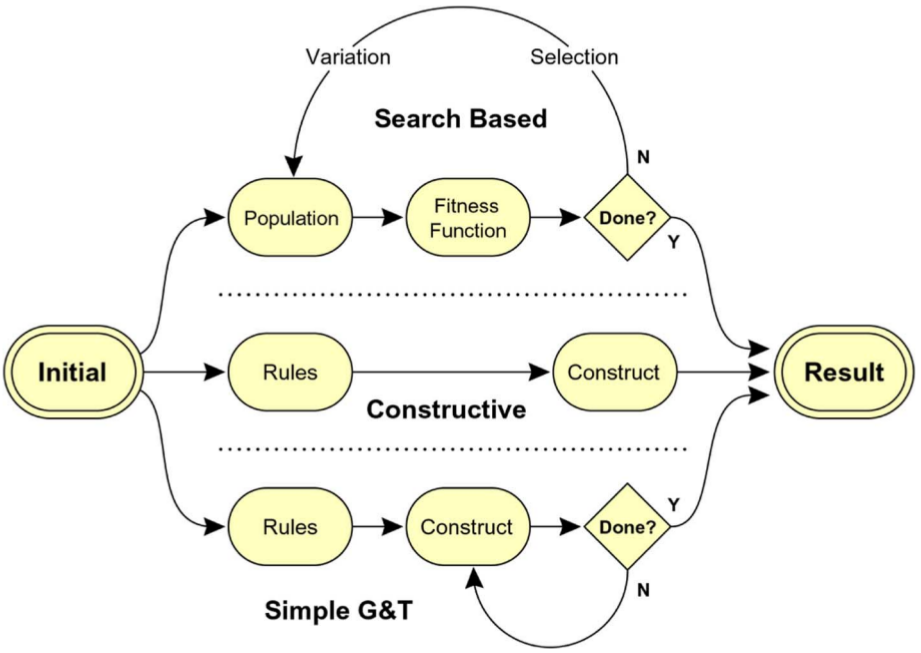
\includegraphics[scale=0.35]{lvlgenmethods}
  \caption{Representation of three types of level generation \cite{5756645}.}
  \label{level}
\end{figure}


\subsection{PCG heuristic techniques}

In each of the approaches above, there exits a difference between deterministic
and stochastic methods of generation. In the former, the generation tool will
generate specified content on each output. In a stochastic method, the results
are somewhat random.

Dormans and Bakkes \@\cite{dormans2011generating} presented a generative grammar
which allows for the generation of levels which are `correct' on a syntactic
level. This was achieved by dividing the content into mission and spaces. The
missions (or game tasks) are generated through the use of recursive, non-linear
graphs. From this output, the structure and shape of the level are constructed
from a separate `shape' grammar. The authors also utilised differing player
models in order to dynamically adjust difficulty, resulting in more adaptive
levels.


To ensure efficient level generation, both Compton and Mateas
\cite{compton2006procedural} and Smith \textit{et al}.
\cite{Smith:2009:RLG:1536513.1536548} generate levels for 2D platform games by
first splitting the levels into smaller sections. From a platform tileset, those
smaller sections could be generated. This is the concept of `rhythm'-based
generation: the pattern is derived from how the game is to be played. This
allows for a range of the types of generated levels as well as maintaining the
pacing of the game \cite{Smith:2009:RLG:1536513.1536548}. The
Figure~\ref{level2} below illustrates the process.

\begin{figure}[h!]

  \centering     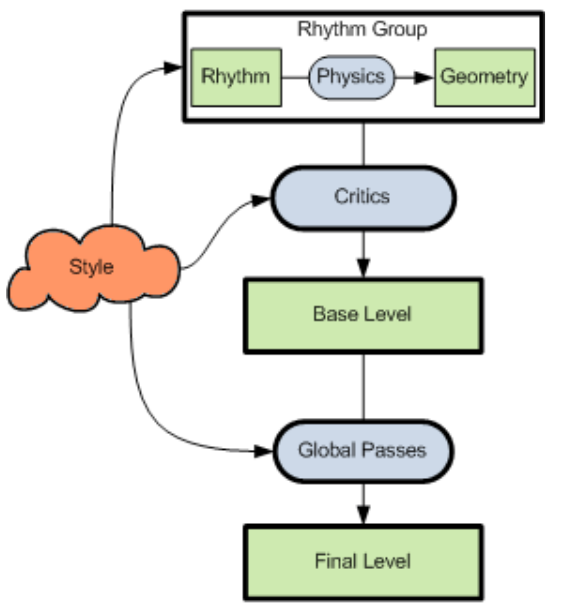
\includegraphics[scale=0.35]{lvlgen}      \caption{Level generation algorithm from
\cite{Smith:2009:RLG:1536513.1536548}. The authors describe the green items as the generated content
and blue boxes as constraints in order to ensure quality generation that adheres to specified
criteria.}  \label{level2} \end{figure}

In a somewhat different fashion, the research from Jennings-Teats \textit{et
al}. \cite{jennings2010polymorph} and Shaker \textit{et al}.
\cite{shaker2010towards} demonstrate that a player's actions can be used for
online generation of platform levels. This would entail that the game would
model itself on the user's own style of playing. This is a more focused
application of the approach used in Dormans' implementation
\cite{dormans2010adventures}, which uses a pre-defined grammar to generate the
mission structure. This is then implemented into the 2D-level using another
grammar to translate this structure.

In a survey on the the evolution of game designs, Togelius and Schmidhuber
\cite{5035629} posit that `fun' in a game is derived from learning how to play
and ultimately mastering the mechanics. While this may be true to an extent
\cite{Burgun:2012}, the declaration and incorporation of these constraints into
an algorithm for generation is limited insofar as the design matches human
experience \cite{sorenson2011generic}.

% Sorenson \textit{et al.} \@\cite{sorenson2011generic} proposed that content generation should  levels
% that is founded on an explicit model of the relationship between challenge and fun. The author
% wanted to increase the fun level of player and the challenges should not bore the human. Therefore
% he modelled a fitness function and levels were designed for \textit{Super Mario Bros} with high
% accuracy. The technique insures that human will generate certain portion by hand and then the model
% used will evaluate the content generated – this evaluation is similar to the evaluation of automatic
% content. The levels will be a mixture of straightforward and difficult portion like the rhythm-group
% structure of high and low nodes, giving games more interesting levels.

Mourato \textit{et al.} \cite{mourato2011automatic} proposed using a genetic
algorithm in order to generate game content for human-players. A genetic
algorithm is a search heuristic that generates approximations through selection
and mutation \cite{srinivas1994genetic}. The authors achieved modest but
positive results including increased level variety and ability to add necessary
and optional content correctly. This method is not entirely suitable for the
current research project as the authors' goals has been to

Smith \textit{et al.} \@\cite{smith2011tanagra} presented a design tool
(TANAGRA) that merged the input from the game designer and the PCG algorithm to
produce levels for a 2D platform game. The technique allowed the designer to
establishes rules and constraints to specify specific content, but allows the
algorithm to decide that which is unspecified. The authors content that this
provides for more diversity in level design as well as enhanced entertainment
value.

A rhythm-based technique is common approach to automatic level generation.
Mawhorter and Mateas \cite{mawhorter2010procedural} devised the `occupancy
regulated extension' algorithm which stitches together samples (referred to
`chunks') authored by human developers into a playable level. This method
described here could be combined with. This is further elaborated upon in the
next chapter on design considerations.

\section{Chapter summary}

Level generation is a dynamic, growing area of video games research. There exist
a number of different methodologies and approaches appropriate for the stated
goals of the research project. For the purposes of the research project, many of
these approaches are not necessarily applicable in initial design and
implementation. Many studies, such as \cite{sorenson2011generic},
\cite{5035629}, and \cite{smith2011tanagra} focus on creating varied content
that is focused on player experience. This may not be an immediate priority in
the research project as the focus is to be able to generate large levels that
correctly represent SAT expressions.

To this end, the rhythm-based approach
\cite{compton2006procedural,Smith:2009:RLG:1536513.1536548} and `chunk approach'
\cite{mawhorter2010procedural} are most pertinent as it would allow various
gadget clauses to be pre-created and joined together to make larger scale levels
to be solved. The creation of an efficient algorithm (even a genetic one
\cite{mourato2011automatic}) represents an area of future research. This will be
further explored in the next chapter on design considerations.


% ------------------------------------------------------------------------------
% CHP 5 --- DESIGN CONSIDERATIONS
% ------------------------------------------------------------------------------

% \chapter{Design Considerations}

% \epigraph{``Design is so simple, that's why it is so complicated.''}{Paul Rand}

% \section{Overview}

% The purpose of this penultimate chapter is to highlight the preliminary design
% considerations and features of the project. The research project being
% undertaken is 66\% Type I (software/hardware development) and therefore it is
% important to address how the discussion in the previous sections affects the
% implementation component. These considerations will form the basis of the
% initial work plan of the project.

% This chapter will first explain the research project's design goals. The
% discussion will then explore the features that have been selected from the
% current research review, highlighting any justifications for design choices.
% Finally, the chapter will identify the next steps.

% \section{Initial software design}

% \subsection{Design goals}

% Recalling the project aims in Chapter 1, the software being developed will
% convert a Boolean formula into a playable 2D platform level. As previously
% mentioned, certain propositional logic formulae are known to be NP-complete.
% This level can then be solved by a SAT solver. The decisions of the SAT solver
% will be converted into moves within the game (i.e. the player character will
% move and address the obstacles). The outcome of this is to allow the
% visualisation of computational complexity, which may have a teaching impact. For
% this to work, the generated levels must look and play as familiar levels for
% students and users of video games.

% The Figure~\ref{project_design} below illustrates the components of the software and how these integrate to achieve the
% research aims.


% \begin{figure}[h!]

%   \centering
%     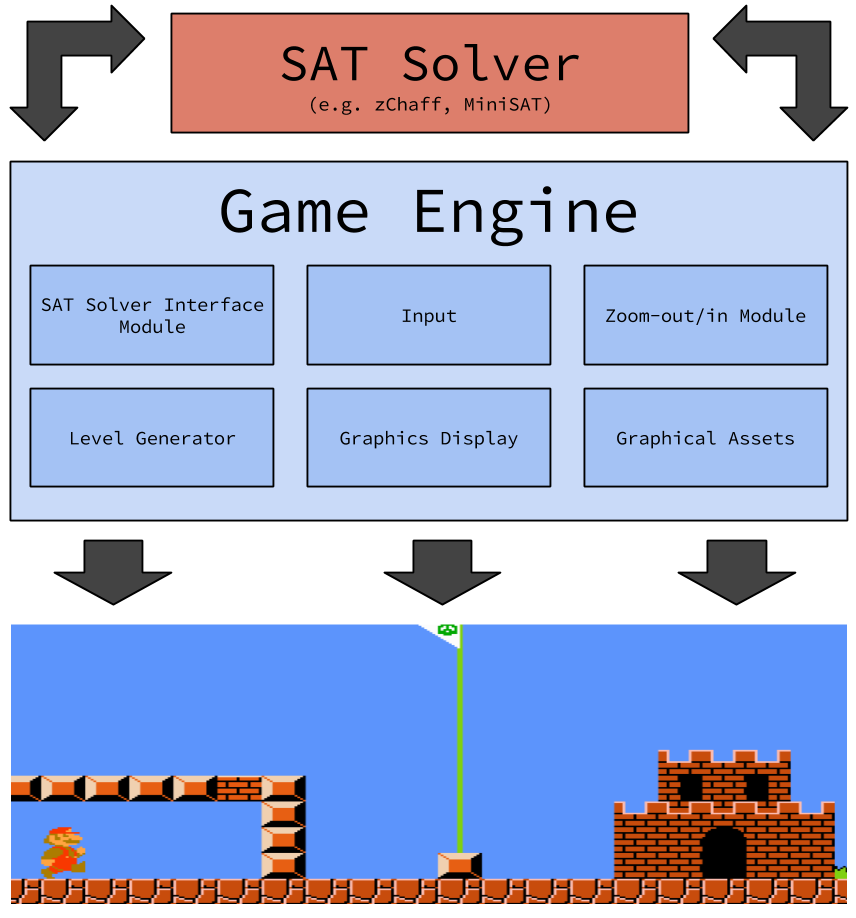
\includegraphics[scale=0.3]{diagram(2)}
%   \caption{Illustrative model for project design. This demonstrates how the modules are grouped and work with the SAT solver to produce the visualisation through a video game medium. Game image adapted from \cite{Aloupis2012}.}
%   \label{project_design}
% \end{figure}

% The `game engine' is comprised of several modules, most significant of which are
% the level generator, the SAT solver interface, and the cluster of models
% managing the graphics and inputs. Furthermore, the game engine should also allow
% for a human player to attempt the level.

% \subsection{Level generation}

% Level generation is a vital component of the research project; the software
% should take an input and convert the SAT instance into which is NP-complete
% (e.g. 3SAT). As the `game' being created is generic, there may be opportunity to
% incorporate elements which classify the level as PSPACE . Using the framework
% provided by Aloupis \textit{et al}. \cite{Aloupis2012}, the computationally hard
% level may be created through deterministic procedural content generation,
% utilising either the `chunk-based' approach proposed by Mawhorter and Mateas
% \cite{mawhorter2010procedural} or the `rhythm'-based approach of Compton and
% Mateas \cite{compton2006procedural} and Smith \textit{et al}.
% \cite{Smith:2009:RLG:1536513.1536548}. This allows for the gadgets to be pre-
% defined and ensures level-generation of a consistent quality. The constraints
% and rules should be quality controlled through the generate- and- test
% methodology.

% \subsubsection{Generating large levels}

% The aim of the research project is to also have large levels that scale to the
% size of the input formula. There are efficiency and quality trade-offs with
% heuristics, such as the genetic algorithm \cite{mourato2011automatic}. This will
% be examined during the implementation of the project and tested for performance
% and efficiency.

% \subsection{Graphical representation}

% One aim of the research project is to generate large scale levels. These levels
% would be many magnitude larger than what an average platformer would contain.
% Therefore, a view adjustment module (or `zooming' module) would be necessary to
% address this in order to help with the visualisation process.


% \subsection{Interfacing with the SAT solver}

% The game engine will have to interface with the chosen SAT solver in order to
% interpret its decisions as player character movements. The concept is to be able
% to visualise how decision- branching operates. The decision trail would be
% colour coded so that a user could see how the solver operated and the steps that
% had been taken.There is scope to allow for multiple SAT solvers to attempt the
% same SAT instance (as depicted in the Figure~\ref{model_project} below). The
% feasibility will be assessed during the development of the software.

% \begin{figure}[h!]

%   \centering
%     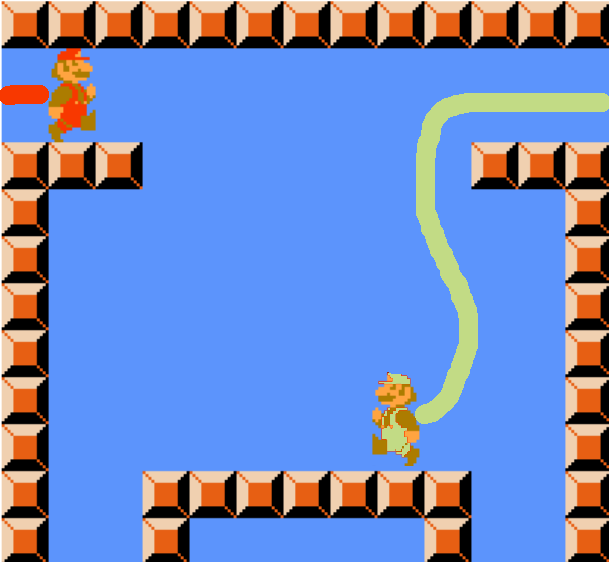
\includegraphics[scale=0.3]{running}
%   \caption{A mock-up of two sat-solvers (represented by the two player characters
% ) simultaneously solving the same level. Image adapted from \cite{Aloupis2012}.}
%   \label{model_project}
% \end{figure}


% \subsection{Human playability}

% There is scope for the software to incorporate an option for playability by
% human users. This would allow for future research in whether the game engine
% produced from this research project could be useful as a teaching tool. This
% question and its implications would be the subject of future work beyond the
% scope of the project. The goal however is to create a tool for such
% investigation and therefore this feature will be included in the initial model
% of the project.


% \section{Use of existing projects}

% There are existing open-source 2D platform games available. While the design
% concept is to create a bespoke software engine that would be able to meet the
% research aims, these games can be utilised as references and models for
% implementing features for the game engine during the development of the research
% project. The two most relevant are listed and considered below.

% \subsection{\textit{Secret Maryo Chronicles}}

% The \textit{Secret Maryo Chronicles} project is an open-source game that models
% itself very closely on the Super Mario Bros franchise \cite{supermaryo}. While,
% there is no longer any active development, the game may act as a reference for
% generating a game engine.

% \subsection{\textit{Nikki and the Robots}}

% \textit{Nikki and the Robots} is an open-source 2D platform game written in
% Haskell \cite{nikki}. The game utilises a level generation function that would
% be of performance interest to the research project. However, as the code is in
% Haskell, this represents a steep learning curve if one is not familiar with the
% language. This is addressed in more detail in the below section.


% \section{Programming language considerations}

% As the research involves a sizeable portion of implementation, it is important
% to include.

% A very significant portion of video games have been and are written in the C/C++
% languages for not only historical reasons but also due to performance
% optimisation and a rich number of application program interfaces (APIs)
% \cite{Gregory:2009}. For the purposes of the research project, the language most
% likely to be used is C++ for the reasons already expressed. Furthermore, as all
% of the listed DPLL-based SAT solvers in Section are written in C or C++ for
% efficiency reasons \cite{zhang2002quest}. Therefore, using C++ should allow for
% easier integration and interoperability.

% \section{Design summary}

% The design incorporates the entirety of the research review's scope, from
% identifying complexity classes to solving Boolean satisfiability instances and
% generating visual game levels based on those instances. Once implemented, the
% game engine will be able to take a SAT instance as an input and generate a level
% in a deterministic, rhythm or chunk based approach. This may naturally change
% during the course of the project as development challenges arise.

% ------------------------------------------------------------------------------
% CHP 6 --- SUMMARY AND CONCLUSIONS
% ------------------------------------------------------------------------------

% \chapter{Conclusions and future work}

% \epigraph{``What we call the beginning is often the end. And to make an end is
% to make a beginning. The end is where we start from.''}{TS Eliot}

% \section{Overview}

% The research review has established a broad theoretical basis from which to
% begin the modelling developing a viable design of the game engine, as
% illustrated in the previous chapter. As a consequence, the implementation and
% development of the game engine design will now be able begin its preliminary
% stages. To this end, the outcome of the research review has been successful and
% its scope complete.

% This however does not mean that the review of literature has been completed for
% the entirety of the research project. The current review will continue to be
% augmented and developed in parallel with the development of the game engine
% software implementation. Already this review has identified new areas of
% investigation in order to complete the research aims of the project. This is
% contained in the future work section below.

% \subsection{Future work}

% \subsubsection{Selection of appropriate SAT features}

% During the implementation, further review and investigation will be conducted
% into the heuristic selection features of SAT solvers. This will be done in order
% to select appropriate solvers which can efficiently interface with the software
% in order to provide for successful visualisation of complexity problems.

% \subsubsection{Ability to run multiple SAT solvers simultaneously}

% An idea that had surfaced was the concept of being able to run two different SAT
% solvers (e.g. zChaff and MiniSAT) simultaneously during a problem instance. The
% literature was not clear on the subject and as such requires further
% investigation and experiment to evaluate whether this could constitute a feature
% of the game engine.

% \subsubsection{Experiments with level generation}

% A greater investigation will be needed once the content generation techniques
% are developed and utilised. At this the current stage, it is not possible to
% know what sort of challenges may arise during implementation, as research has
% been solely based on heuristic models.

% \subsubsection{Identification of further complexity classes}

% After the successful integration of software features, the literature review
% will benefit from identifying other possible classes of complexity that could be
% tested within the developed software.



% ------------------------------------------------------------------------------
% Level Design and Generation
% ------------------------------------------------------------------------------

\chapter{Level Design and Generation}

In the previous chapters, the basis for making a 2D platform game NP-hard was 
established. In this chapter, the focus will be on designing a playable level 
that incorporates those elements. 

In previous literature, the level design has focused on the gadgets that
correspond to 3SAT reductions in order to prove that the game is in
fact NP-hard.. In these models, the actual gameplay is
generalised and left-otherwise unaddressed. 

This provides a challenge when 

\section{Designing NP-hard levels}

For the purposes of this project, the size of the levels are n X n, which 
means that the size is essentially unlimited. 

% Review Aloupis and Forisek

% \section{Modifying the model in Aloupis \textit{et al}}

% The Aloupis et al model 

% \subsection{Modification 1: Joining the variable with the clause}

% In the A model, the player assigns a value to variable by deciding to fall down
% one side or another. The fall leads to a clause where that literal resides. The
% player then renders the clause TRUE by performing the action. In reality, it
% does not matter whether the

% \subsection{Modification 2: Progressing to the next variable assignment}

% This issue was addressed by utilising the warp pipes in \textit{Super Mario
% Bros.} In the game, the player can make use of certain pipes to travel either to
% different areas  of the level that would otherwise not be accessible or to other
% levels entirely.

% The use of warp tunnels has two functions: (1) it allows for a neat way in which 
% to demonstrate clauses

% In the Aloupis model, the need for enemies does not feature as prominently as
% with  Forisek. Forisek contends that enemies are required in order to

% \subsection{Modification 3: Preventing cross-over}

Figure ~\ref{full-level}demonstrates how the gadgets may be phsyically linked
together in a three variable, three clause 3SAT reducation.

\begin{figure}[ht!]

  \centering
    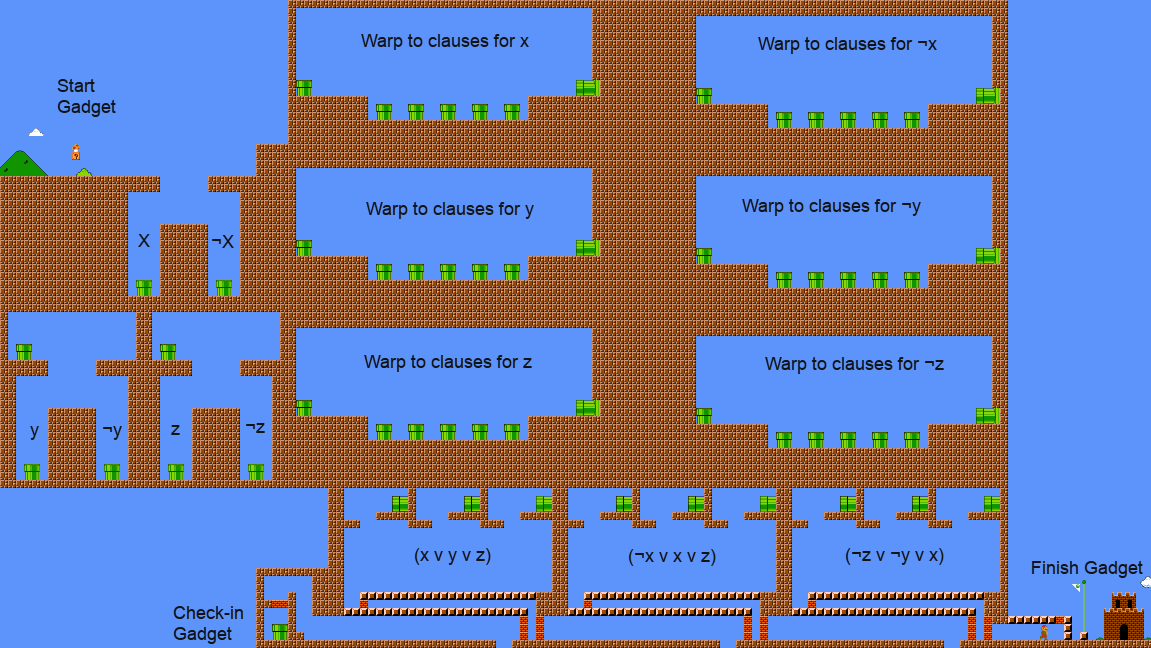
\includegraphics[scale=0.25]{fulllevel-text}
  \caption{Representation of physical linking of gadgets.}
  \label{full-level}
\end{figure}

This will be briefly described below. 

The player starts as in Aloupis et al \cite{Aloupis2012} with a start gadget
that turns `small' Mario (composed of a single 16x16 tile) into Super Mario.
Super Mario can jump under bricks and break certain types of blocks. Once
sufficiently progressed to the right, the screen view will bring the first
variable gadget into focus.

The variable gadget relies on the meta-theorem provided by Fori\v{s}ek
\cite{DBLP:conf/fun/Forisek10} (long fall). In Aloupis et al \cite{Aloupis2012},
the authors created a cross-over gadget that prevented the player from by-
passing or accessing areas of the level which impact the reducation to a 3SAT
instance. The authors are not entirely clear exactly how the gadgets are
physically linked together. This presentes a number of challenges when scaling a
level. In Aloupis, the 3SAT instance has three clauses. However, when dealing
the amount of cross over increases.

There are a number of issues which arise when scaling a level.

In \textit{Super Mario Bros.}, the player may discover that certain pipes are
able to be utilised in order to travel to different hidden areas or even other
levels. This game mechanic provides a useful solution to scalability. 

In the project's implementation, after the player picks a variable by falling
and using the pipe, the player is taken to a clause choosing gadget. Here there
are a series of pipes, each leading to a particular clause where the literal
appears.

\begin{figure}[ht!]

  \centering
    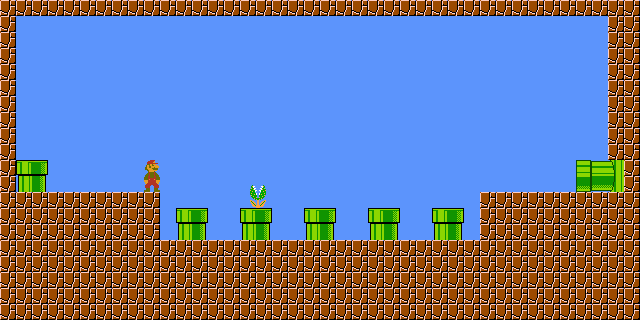
\includegraphics[scale=0.70]{clause}
    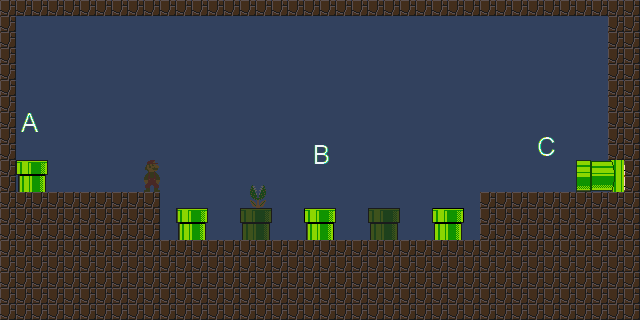
\includegraphics[scale=0.70]{clause-explain}
  \caption{Crossing into other clause areas.}
  \label{clause-crossing}
\end{figure}

% \begin{figure}[ht!]

%   \centering
%     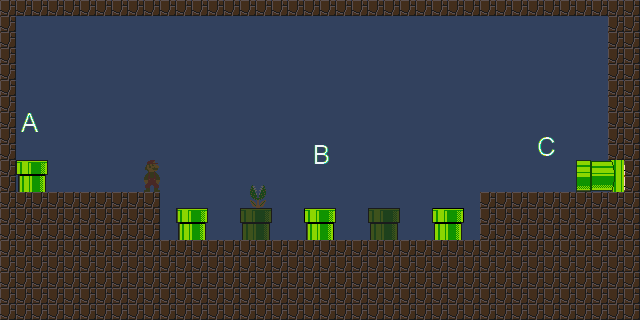
\includegraphics[scale=0.70]{clause-explain}
%   \caption{Crossing into other clause areas.}
%   \label{clause-crossing-explain}
% \end{figure}

In the clause-crossing gadget, the player enters on the pipe on the left (marked
A). The player is not able to return through this pipe. Even if it was the case,
the player cannot overcome the variable gadget.

There are five pipes of which three lead to clauses and the other two contain
\textit{Piranha plants}, venus-fly trap like enemies in \textit{Super Mario
Bros} (Marked B). Once the clauses have been visited and unlocked, the player
returns through the pipe on the right side of the screen (marked C) and can
proceed to the next variable assignment. If the player has no more variable
assignments to make, the pipe will lead to the check-in gadget, illustrated in
Figure~\ref{check-in}. The check-in gadget allows the player to progress through
the check-out and ultimately to the finish gadget.

\begin{figure}[ht!]

  \centering
    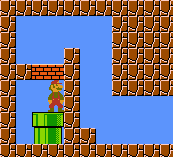
\includegraphics[scale=1.2]{check-out}
  \caption{The check-in gadget. Note the player can only advance as Super Mario.}
  \label{check-in}
\end{figure}

Once the player checks-in, the player then advances through the check-out of the
level. The check-out phase is only passable if the clauses have been opened. The
only obstacle at this point of the game is the drop in the floor. The player
then proceeds to the finish gadget, shown in Figure~\ref{finish}.

\begin{figure}[ht!]

  \centering
    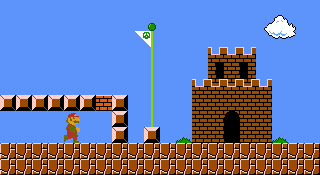
\includegraphics[scale=1.0]{finish}
  \caption{The check-in gadget. Note the player can only advance as Super Mario.}
  \label{finish}
\end{figure}










% ------------------------------------------------------------------------------
% Game Engine Design
% ------------------------------------------------------------------------------

\chapter{Game Engine Design}

\section{Design considerations}

\subsection{Development language and libraries}

The game was developed in C++ using the C++11 standard. The C++ language was
selected because this is the same language used in the source code for SAT
solvers. This ensures that the code base can easily be adapted into the game
engine without the need to develop an API or wrapper, which would have detracted
from time developing the game engine.

The game engine uses the Simple and Fast Media Library (SFML) for handling
graphics and player input. There are a number of libraries which can provide this
functionality. The primary criteria in selecting a suitable multimedia library
was based on ease of use and ease of integration. 

The candidate libraries were SFML, SDL, and Allegro, as these were the most
popular choices for C++ game development. The decision to use SFML was based on
the use of C++. SFML distinguishes itself from the other two libraires in that
it is written for C++ and thereby provinding a way to use the multimedia library
in an object-orientated fashion. Another strong choice was SDL. However, SDL
lacks the support for object-orientation that SFML provides. At any rate, the
multimedia library is not of any significant impact or consequence.

The game was developed on Ubuntu Linux 15.04 with SPECS. It was compiled using
LLVM/Clang (clang++). There is no appreciable difference when using the GNU
Compiler Collection (gcc). Instructions to switch the makefile to gcc rather
than clang++ are contained in the wiki as well as the comments within the
project's makefile.

The coding style used for the development was the Google C++ style guide. The
intention is that this research will continue to be developed after this
project's completion and  that future work may be continued on the same code
base. This particular style guide was chosen because it is widely available and
provides good references.

\section{Basic game engine mechanics}

\subsection{Game loop}

\subsection{Player movement}

\subsection{Collision management}

\section{Level generation}

The levels are drawn using a tile-based method. There are a number of methods
that could be used

\section{SAT solver integration}

The Game State Manager class has a private member called
\texttt{SAT\textunderscore Manager\textunderscore} which integrates the zchaff
SAT solver into the game engine.

\subsection{Reading in the CNF file}

\subsection{Accessing variables and clauses}

\section{Project wiki and references}

A project wiki has acted as a journal and reference guide for the game engine's 
development. The rationale behind keeping this documentation was to allow for 
future development work to be carried out on the game engine. 

\section{Unit testing}

The game engine source code also includes a testing framework for the various
modules. In this project, googletest, Google's C++ Testing Framework was used. 

% ------------------------------------------------------------------------------
% EVALUATION
% ------------------------------------------------------------------------------

\chapter{Evaluation}

% \section{Use of C++}

% The use of C++ as the development language is good. There are others but C++
% allows for scalability.

% There is scope for procedurally generating content using other languages. One
% explored was Haskell.

% \section{Use of Haskell to generate content}

% ------------------------------------------------------------------------------
% FUTURE WORK
% ------------------------------------------------------------------------------

\chapter{Future Work}

\section{Constrained level size}

% A level that is 14 x 14 tiles as the original SMB was.

\section{Additional complexity classes}

\subsection{PSPACE}

\subsection{EXSPACE}

\section{Web Deployment}

% ------------------------------------------------------------------------------
% BIBLIOGRAPHY
% ------------------------------------------------------------------------------

\bibliographystyle{abbrv}
\bibliography{../ResearchReview/references.bib}

\end{document}
